\documentclass[landscape,a0b,final,a4resizeable]{a0poster}
%\documentclass[landscape,a0b,final]{a0poster}
%% orange2 で作成する場合は,
%%   (1) platex poster2
%%   (2) dvipdfm poster2       (または dvipdfmx poster2 ; PDF の生成)
%%   (3) acroread poster2.pdf 
%% Mac の TeXShop でも作成できます.
%% 仕上げは必ず orange でやる.
%%   (1) platex poster2  (これをもう一度やらないと ps2pdf でエラーに)
%%   (2) dvips poster2  (poster2.ps が生成される)
%%   (3) ps2pdf poster2.ps  (poster2.pdf が生成される)
%%   (4) acroread poster2.pdf
%% 次のコメントよく読んで下さい.
%\documentclass[portrait,a0b,final]{a0poster}
%%% Option "a4resizeable" makes it possible ot resize the
%   poster by the command: psresize -pa4 poster.ps poster-a4.ps
%   For final printing, please remove option "a4resizeable" !!
% これは今うまく動きません.
%%  platex poster2
%%  dvips poster2 >t.ps
%%  psresize -pa4 t.ps tt.ps
%%  lpr -Pxerox-3s tt.ps で A4 用紙に試し印刷.
%%  lpr -Pxerox-4s tt.ps で A4 用紙に試し印刷 (カラー)

\usepackage{epsfig}
\usepackage{multicol}
\usepackage{pstricks,pst-grad}
\usepackage{newrgb}   %% いろんな色を使うため. 色の一覧は newrgb.sty を見よ.

%%%%%%%%%%%%%%%%%%%%%%%%%%%%%%%%%%%%%%%%%%%%%%
%% 以下のマクロ定義等はそのまま使う. いじらない.
%%%%%%%%%%%%%%%%%%%%%%%%%%%%%%%%%%%%%%%%%%%
% Definition of some variables and colors
%\renewcommand{\rho}{\varrho}
%\renewcommand{\phi}{\varphi}
\setlength{\columnsep}{3cm}
\setlength{\columnseprule}{2mm}
\setlength{\parindent}{0.0cm}


%%%%%%%%%%%%%%%%%%%%%%%%%%%%%%%%%%%%%%%%%%%%%%%%%%%%
%%%               Background                     %%%
%%%%%%%%%%%%%%%%%%%%%%%%%%%%%%%%%%%%%%%%%%%%%%%%%%%%

\newcommand{\background}[3]{
  \newrgbcolor{cgradbegin}{#1}
  \newrgbcolor{cgradend}{#2}
  \psframe[fillstyle=gradient,gradend=cgradend,
  gradbegin=cgradbegin,gradmidpoint=#3](0.,0.)(1.\textwidth,-1.\textheight)
}



%%%%%%%%%%%%%%%%%%%%%%%%%%%%%%%%%%%%%%%%%%%%%%%%%%%%
%%%                Poster                        %%%
%%%%%%%%%%%%%%%%%%%%%%%%%%%%%%%%%%%%%%%%%%%%%%%%%%%%

\newenvironment{poster}{
  \begin{center}
  \begin{minipage}[c]{0.98\textwidth}
}{
  \end{minipage} 
  \end{center}
}



%%%%%%%%%%%%%%%%%%%%%%%%%%%%%%%%%%%%%%%%%%%%%%%%%%%%
%%%                pcolumn                       %%%
%%%%%%%%%%%%%%%%%%%%%%%%%%%%%%%%%%%%%%%%%%%%%%%%%%%%

\newenvironment{pcolumn}[1]{
  \begin{minipage}{#1\textwidth}
  \begin{center}
}{
  \end{center}
  \end{minipage}
}



%%%%%%%%%%%%%%%%%%%%%%%%%%%%%%%%%%%%%%%%%%%%%%%%%%%%
%%%                pbox                          %%%
%%%%%%%%%%%%%%%%%%%%%%%%%%%%%%%%%%%%%%%%%%%%%%%%%%%%

\newrgbcolor{lcolor}{0. 0. 0.80}
\newrgbcolor{gcolor1}{1. 1. 1.}
\newrgbcolor{gcolor2}{.80 .80 1.}

\newcommand{\pbox}[4]{
\psshadowbox[#3]{
\begin{minipage}[t][#2][t]{#1}
#4
\end{minipage}
}}



%%%%%%%%%%%%%%%%%%%%%%%%%%%%%%%%%%%%%%%%%%%%%%%%%%%%
%%%                myfig                         %%%
%%%%%%%%%%%%%%%%%%%%%%%%%%%%%%%%%%%%%%%%%%%%%%%%%%%%
% \myfig - replacement for \figure
% necessary, since in multicol-environment 
% \figure won't work

\newcommand{\myfig}[3][0]{
\begin{center}
  \vspace{1.5cm}
  \includegraphics[width=#3\hsize,angle=#1]{#2}
  \nobreak\medskip
\end{center}}



%%%%%%%%%%%%%%%%%%%%%%%%%%%%%%%%%%%%%%%%%%%%%%%%%%%%
%%%                mycaption                     %%%
%%%%%%%%%%%%%%%%%%%%%%%%%%%%%%%%%%%%%%%%%%%%%%%%%%%%
% \mycaption - replacement for \caption
% necessary, since in multicol-environment \figure and
% therefore \caption won't work

%\newcounter{figure}
\setcounter{figure}{1}
\newcommand{\mycaption}[1]{
  \vspace{0.5cm}
  \begin{quote}
    {{\sc Figure} \arabic{figure}: #1}
  \end{quote}
  \vspace{1cm}
  \stepcounter{figure}
}



%%%%%%%%%%%%%%%%%%%%%%%%%%%%%%%%%%%%%%%%%%%%%%%%%%%%%%%%%%%%%%%%%%%%%%
%%% Begin of Document
%%%%%%%%%%%%%%%%%%%%%%%%%%%%%%%%%%%%%%%%%%%%%%%%%%%%%%%%%%%%%%%%%%%%%%

\begin{document}

\background{1. 1. 1.}{1. 1. 1.}{0.5}

\vspace*{2cm}


\newrgbcolor{lightblue}{0. 0. 0.80}
\newrgbcolor{white}{1. 1. 1.}
\newrgbcolor{whiteblue}{.80 .80 1.}


\begin{poster}

%%%%%%%%%%%%%%%%%%%%%
%%% Header   表題.
%%%%%%%%%%%%%%%%%%%%%
\begin{center}
\begin{pcolumn}{0.98}

\pbox{0.95\textwidth}{}{linewidth=2mm,framearc=0.3,linecolor=lightblue,fillstyle=gradient,gradangle=0,gradbegin=white,gradend=whiteblue,gradmidpoint=1.0,framesep=1em}{

%%% Unisiegel
%%% Titel
\begin{minipage}[c][9cm][c]{0.78\textwidth}
  \begin{center}
    {\sc \Huge This is the Title of your Poster}\\[10mm]
    {\Large My Name\\[7.5mm]    
    神戸大学理学系研究科数学専攻 修士1年}
  \end{center}
\end{minipage}
%%% GK-Logo
\begin{minipage}[c][9cm][c]{0.1\textwidth}
  \begin{center}
     %自分の顔写真:   jpeg2ps コマンドで eps ファイルを作成.
    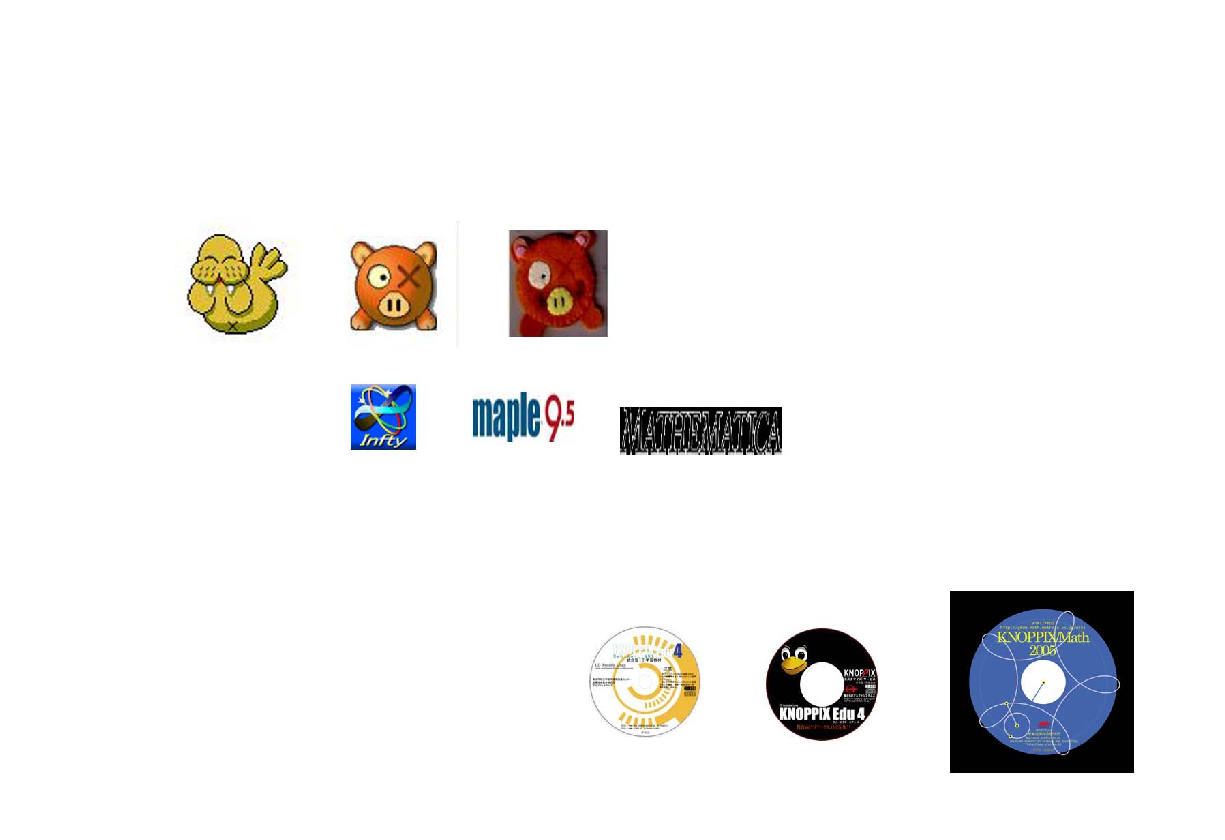
\includegraphics[width=7cm,angle=0]{hopo-inobuta-j.eps}
  \end{center}
\end{minipage}

}
\end{pcolumn}
\end{center}


\vspace*{2cm}



%%%%%%%%%%%%%%%%%%%%%
%%% Content  本文のはじまり.
%%%%%%%%%%%%%%%%%%%%%

%%% Begin of Multicols-Enviroment  3 コラムでのプレゼンテーション.
\begin{multicols}{3}

%%% Abstract
\begin{center}\pbox{0.8\columnwidth}{}{linewidth=2mm,framearc=0.1,linecolor=lightblue,fillstyle=gradient,gradangle=0,gradbegin=white,gradend=whiteblue,gradmidpoint=1.0,framesep=1em}{\begin{center}要約\end{center}}\end{center}
\vspace{1.25cm}

This is your abstract of this poster.
{\DarkBlue これはこのポスター発表の要約}


%%% Introduction
\vspace{2cm}\begin{center}\pbox{0.8\columnwidth}{}{linewidth=2mm,framearc=0.1,linecolor=lightblue,fillstyle=gradient,gradangle=0,gradbegin=white,gradend=whiteblue,gradmidpoint=1.0,framesep=1em}{\begin{center}はじめに\end{center}}\end{center}\vspace{1.25cm}

This is an introduction.
これはイントロダクション.

%%% Section   次の行は節を加える事にコピーして使う.
\vspace{2cm}\begin{center}\pbox{0.8\columnwidth}{}{linewidth=2mm,framearc=0.1,linecolor=lightblue,fillstyle=gradient,gradangle=0,gradbegin=white,gradend=whiteblue,gradmidpoint=1.0,framesep=1em}{\begin{center}Section 1\end{center}}\end{center}\vspace{1.25cm}

これは section 1.
{\DarkBlue This is section 2.}

自分は \cite{abc} の勉強から始めた.

次の定理が成り立つ. \\
{\bf 定理} xxx yyy


%%% Figures:
\begin{center}
  % first argument: eps-file
  % second argument: stretching-factor relative to Column-width (<1)
  % optional argument: rotation angle (0-360), default=0
  \myfig[60]{hopo-inobuta-j.eps}{0.15}
  \mycaption{いのぶた君}
\end{center}

この図は xxx yyy の様子をよく説明している.
この図は xxx yyy の様子をよく説明している.
この図は xxx yyy の様子をよく説明している.


%%% Section
\vspace{2cm}\begin{center}\pbox{0.8\columnwidth}{}{linewidth=2mm,framearc=0.1,linecolor=lightblue,fillstyle=gradient,gradangle=0,gradbegin=white,gradend=whiteblue,gradmidpoint=1.0,framesep=1em}{\begin{center}Section 2\end{center}}\end{center}\vspace{1.25cm}

This is section 2.
論文 \cite{xyz} によると, かくかくしかじか.
論文 \cite{xyz} によると, かくかくしかじか.
論文 \cite{xyz} によると, かくかくしかじか.
論文 \cite{xyz} によると, かくかくしかじか.

%%% Section
\vspace{2cm}\begin{center}\pbox{0.8\columnwidth}{}{linewidth=2mm,framearc=0.1,linecolor=lightblue,fillstyle=gradient,gradangle=0,gradbegin=white,gradend=whiteblue,gradmidpoint=1.0,framesep=1em}{\begin{center}Section 3\end{center}}\end{center}\vspace{1.25cm}

This is section 3.
{\OrangeRed ここは第3章.}


%%% References
%\bibliographystyle{alpha}
%\bibliography{poster.bib}
\begin{thebibliography}{99}
\bibitem{abc} 著者, 本の題名, 発行年, 出版者. 
\bibitem{xyz} 著者, 論文題名, 雑誌名, 巻号 (発行年), はじまりのページ--終りのページ.
\end{thebibliography}


\end{multicols}

\end{poster}

\end{document}

